%
\hsection{Installing LibreOffice under Microsoft Windows}%
%
\begin{figure}%
\centering%
%
\subfloat[][%
We open a web browser and go to \url{https://libreoffice.org}. %
There, we click on \menu{DOWNLOAD}.%
\label{fig:installingLibreOfficeWindows01website}%
]{\tightbox{
\includegraphics[width=0.7\linewidth]{\currentDir/installingLibreOfficeWindows01website}}}%
%
\floatRowSep%
%
\subfloat[][%
In the menu that opens, we click on~\menu{Download LibreOffice}.%
\label{fig:installingLibreOfficeWindows02download}%
]{\tightbox{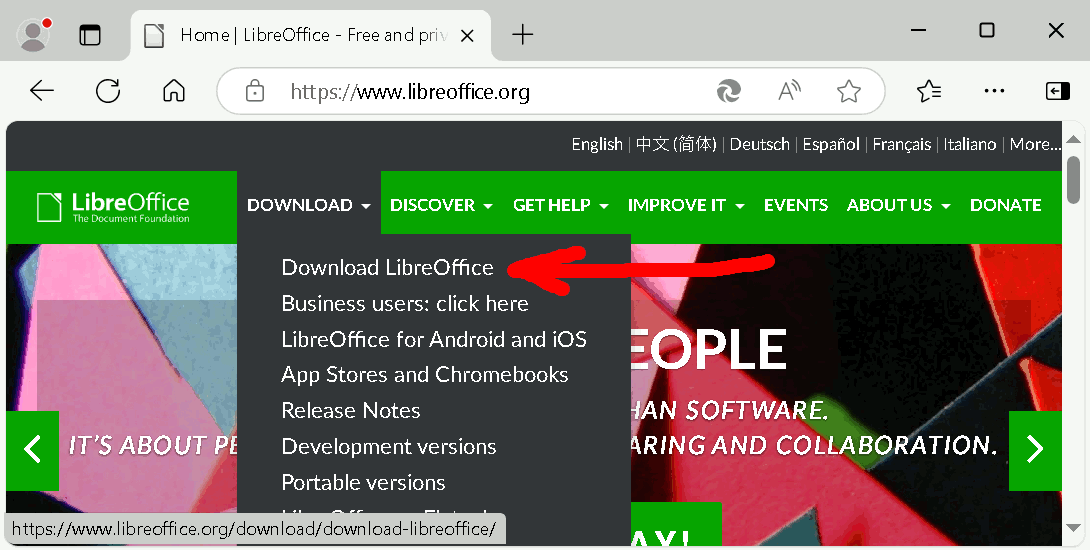
\includegraphics[width=0.7\linewidth]{\currentDir/installingLibreOfficeWindows02download}}}%
%
\floatRowSep%
%
\subfloat[][%
This takes us to the download page, where we click \menu{DOWNLOAD}. %
(We can leave the operator system at the default \menu{Windows (64-bit)} setting.)%
\label{fig:installingLibreOfficeWindows03downloadPage1}%
]{\tightbox{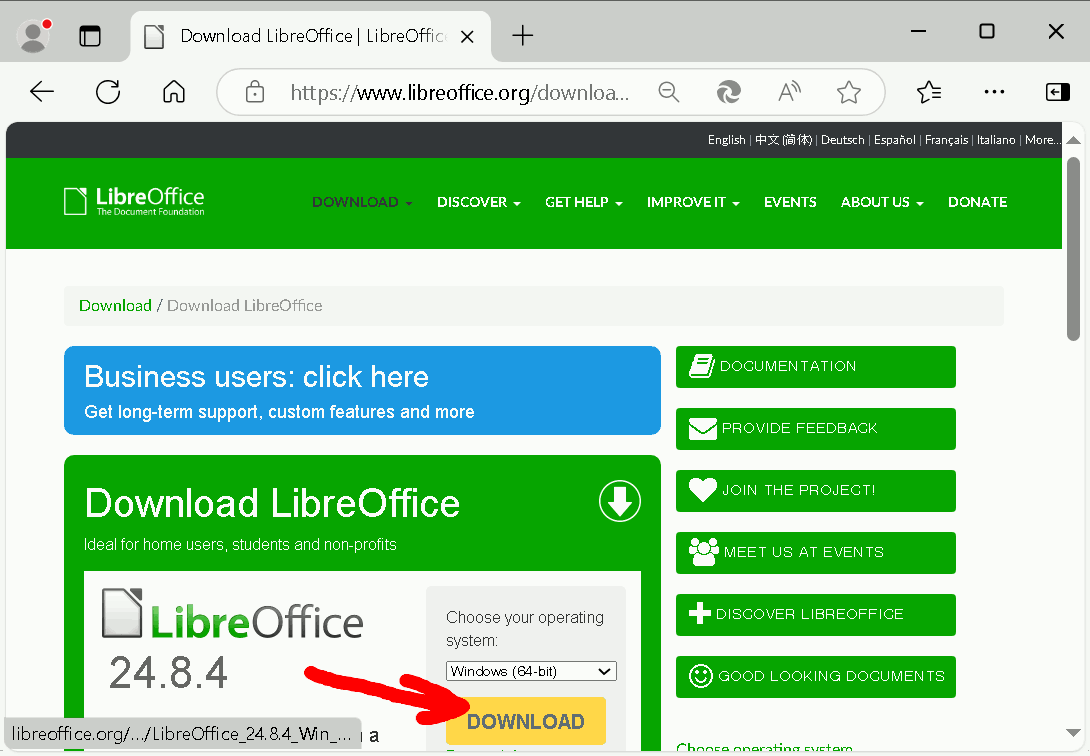
\includegraphics[width=0.7\linewidth]{\currentDir/installingLibreOfficeWindows03downloadPage1}}}%
%
\caption{Installing \libreoffice\ under \microsoftWindows.}%
\label{fig:installingLibreOfficeWindowsA}%
\end{figure}%
%
\begin{figure}%
\ContinuedFloat%
\centering%
%
\subfloat[][%
This takes us to yet another download page, where we click the big button for downloading \libreoffice.%
\label{fig:installingLibreOfficeWindows04downloadPage2}%
]{\tightbox{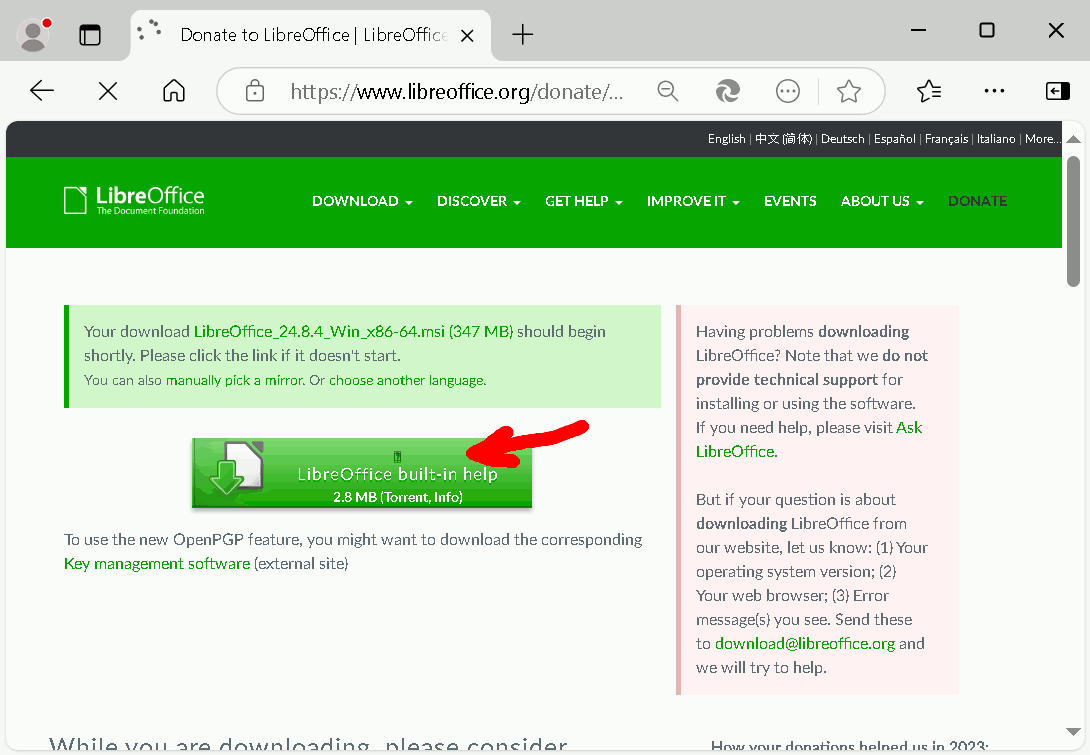
\includegraphics[width=0.7\linewidth]{\currentDir/installingLibreOfficeWindows04downloadPage2}}}%
%
\floatRowSep%
%
\subfloat[][%
The download starts.%
\label{fig:installingLibreOfficeWindows05downloading}%
]{\tightbox{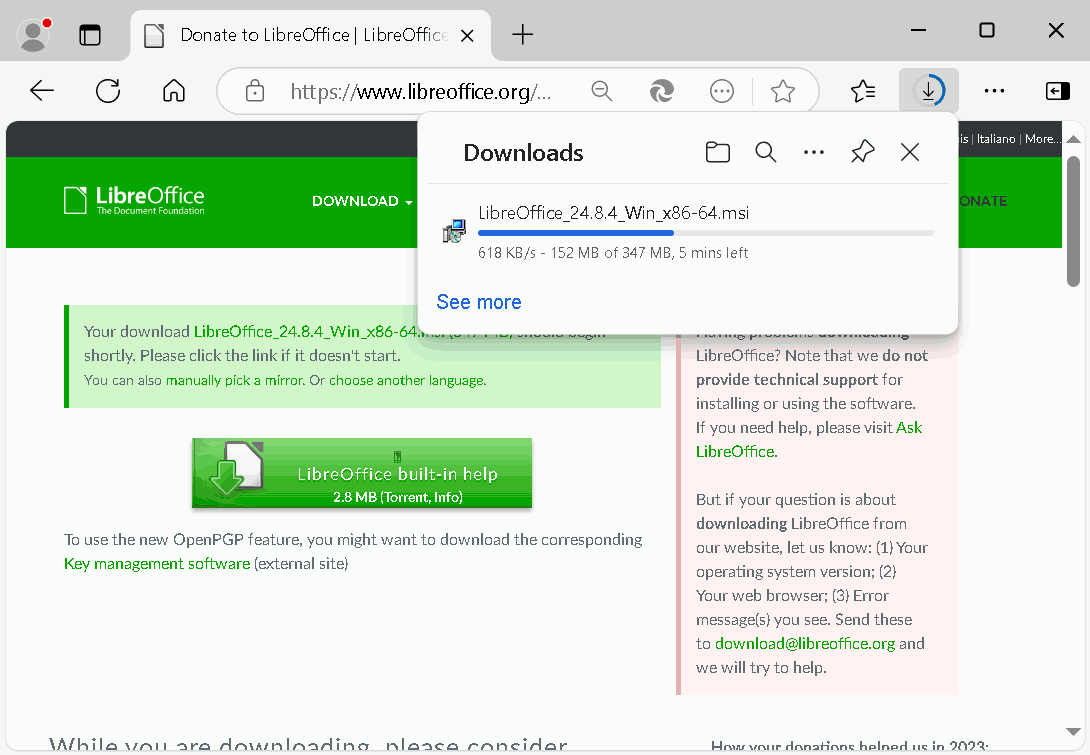
\includegraphics[width=0.7\linewidth]{\currentDir/installingLibreOfficeWindows05downloading}}}%
%
\caption{Installing \libreoffice\ under \microsoftWindows~(Continued).}%
\label{fig:installingLibreOfficeWindowsB}%
\end{figure}%
%
%
\begin{figure}%
\ContinuedFloat%
\centering%
%
\subfloat[][%
After the download completes, we click \menu{Open file}.%
\label{fig:installingLibreOfficeWindows06open}%
]{\tightbox{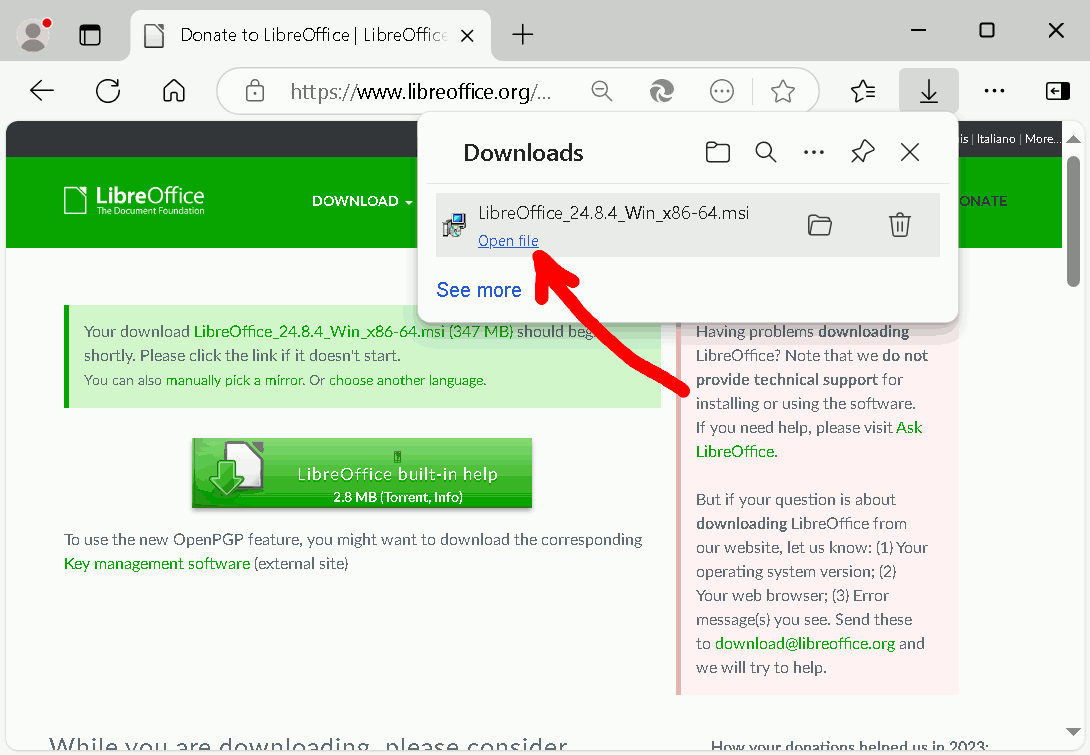
\includegraphics[width=0.7\linewidth]{\currentDir/installingLibreOfficeWindows06open}}}%
%
\floatRowSep%
%
\subfloat[][%
A \microsoftWindows\ loading screen appears.%
\label{fig:installingLibreOfficeWindows07starting}%
]{\tightbox{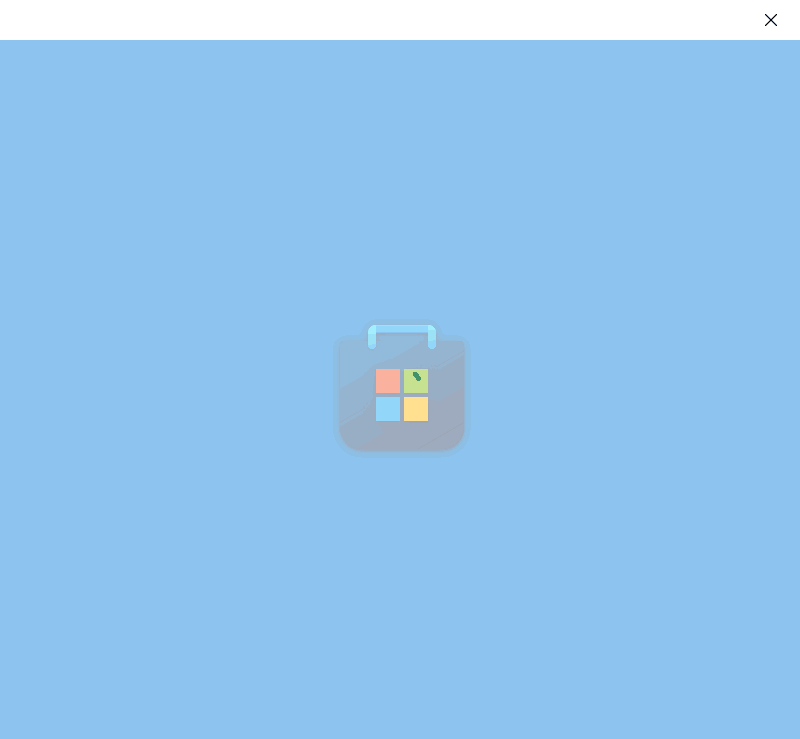
\includegraphics[width=0.315\linewidth]{\currentDir/installingLibreOfficeWindows07starting}}}%
%
\floatSep%
%
\subfloat[][%
We get asked whether we really want to install this program\dots%
\label{fig:installingLibreOfficeWindows08msStore1}%
]{\tightbox{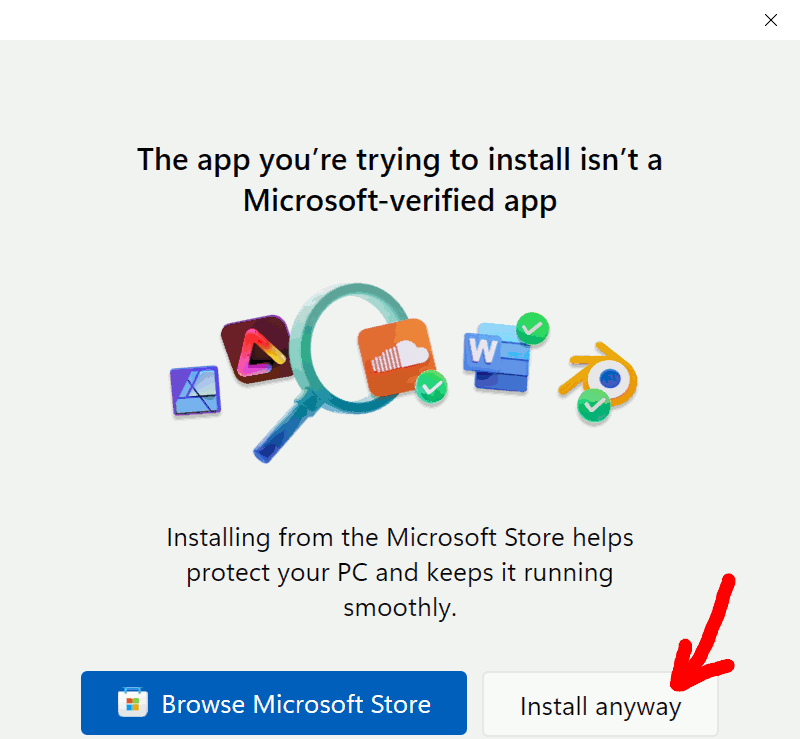
\includegraphics[width=0.315\linewidth]{\currentDir/installingLibreOfficeWindows08msStore1}}}%
%
\floatSep%
%
\subfloat[][%
{\dots}and we click~\menu{Install anyway}.%
\label{fig:installingLibreOfficeWindows09msStore2}%
]{\tightbox{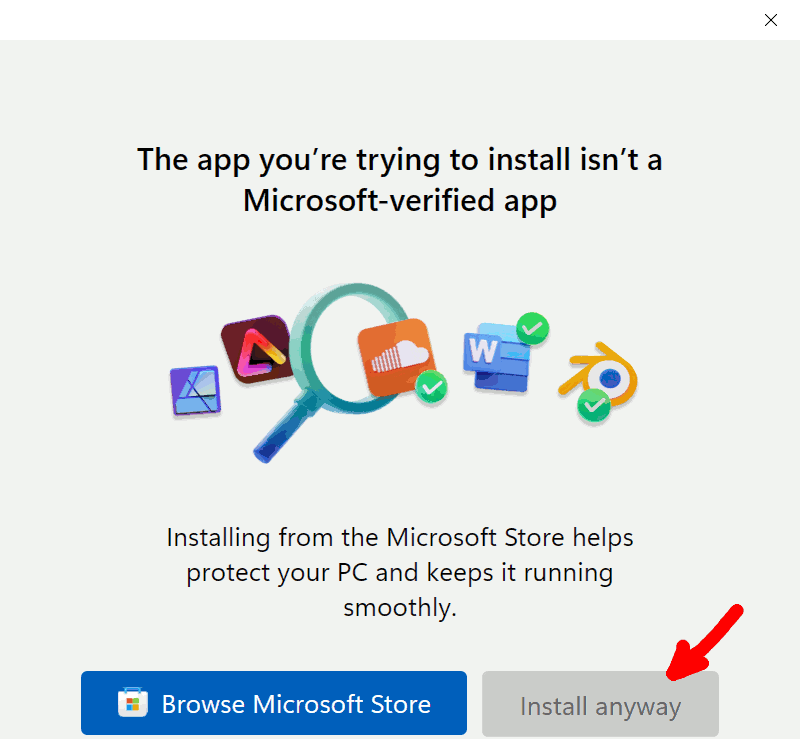
\includegraphics[width=0.315\linewidth]{\currentDir/installingLibreOfficeWindows09msStore2}}}%
%
\floatRowSep%
%
\subfloat[][%
The installation wizard window appears and we click~\menu{Next}.%
\label{fig:installingLibreOfficeWindows10wizard}%
]{\tightbox{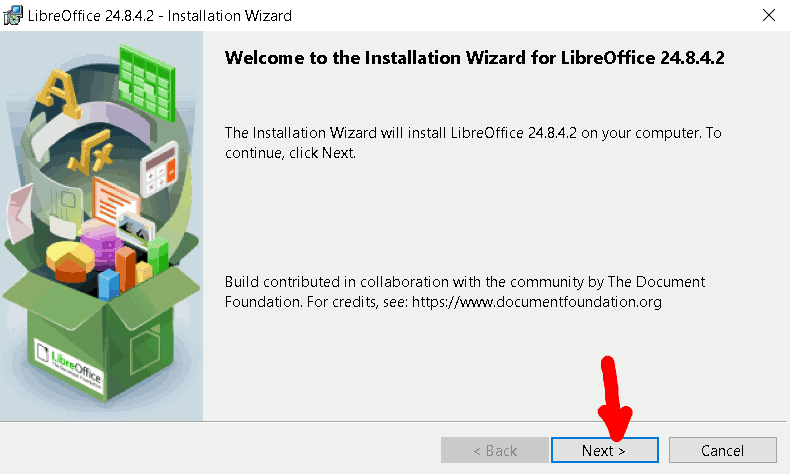
\includegraphics[width=0.7\linewidth]{\currentDir/installingLibreOfficeWindows10wizard}}}%
%
%
\caption{Installing \libreoffice\ under \microsoftWindows~(Continued).}%
\label{fig:installingLibreOfficeWindowsC}%
\end{figure}%
%
%
\begin{figure}%
\ContinuedFloat%
\centering%
%
\subfloat[][%
We are totally fine with a \inQuotes{typical} installation and click~\menu{Next}.%
\label{fig:installingLibreOfficeWindows11wizardTypical}%
]{\tightbox{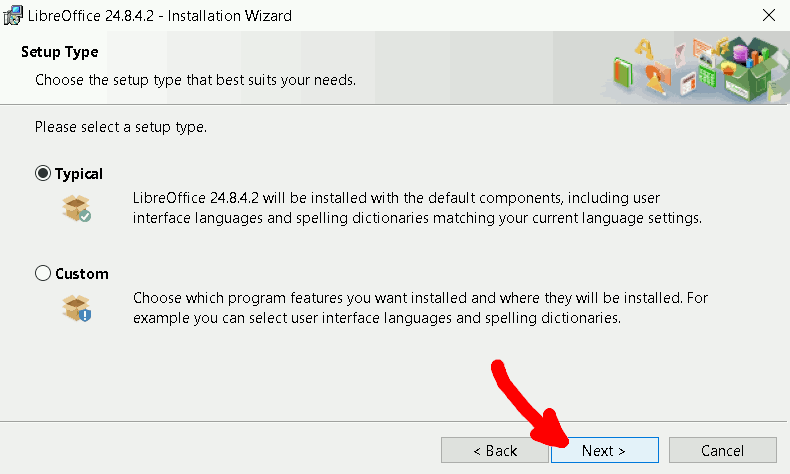
\includegraphics[width=0.7\linewidth]{\currentDir/installingLibreOfficeWindows11wizardTypical}}}%
%
\floatRowSep%
%
\subfloat[][%
We are also OK with a shortcut on our desktop and click~\menu{Install}.%
\label{fig:installingLibreOfficeWindows12wizardStartInstall}%
]{\tightbox{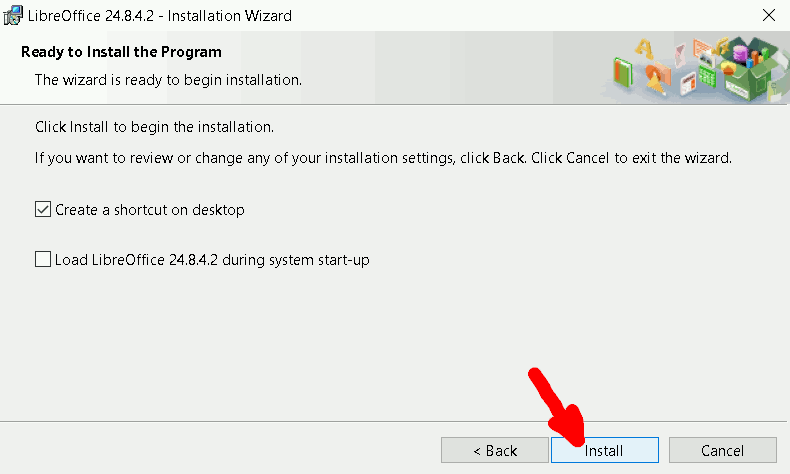
\includegraphics[width=0.7\linewidth]{\currentDir/installingLibreOfficeWindows12wizardStartInstall}}}%
%
\floatRowSep%
%
\subfloat[][%
The installation begins.%
\label{fig:installingLibreOfficeWindows13installStart}%
]{\tightbox{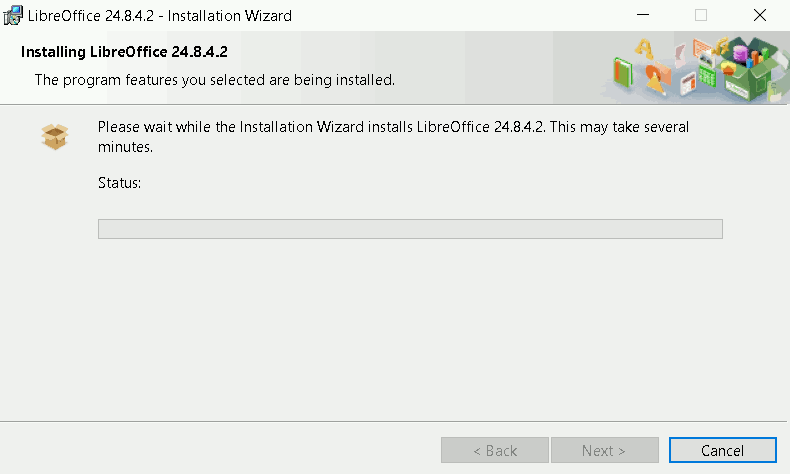
\includegraphics[width=0.7\linewidth]{\currentDir/installingLibreOfficeWindows13installStart}}}%
%
\caption{Installing \libreoffice\ under \microsoftWindows~(Continued).}%
\label{fig:installingLibreOfficeWindowsD}%
\end{figure}%
%
%
\begin{figure}%
\ContinuedFloat%
\centering%
%
\subfloat[][%
\microsoftWindows\ asks us whether we would like to permit the installer to make changes to our system. %
Yes, we are, so we click~\menu{Yes}.%
\label{fig:installingLibreOfficeWindows14permitChanges}%
]{\tightbox{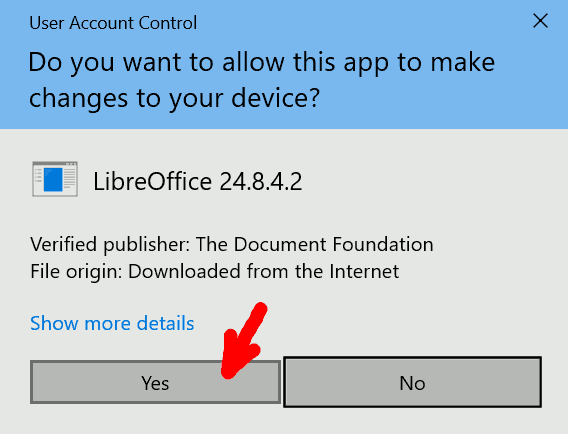
\includegraphics[width=0.55\linewidth]{\currentDir/installingLibreOfficeWindows14permitChanges}}}%
%
\floatRowSep%
%
\subfloat[][%
The installation continues.%
\label{fig:installingLibreOfficeWindows15installing}%
]{\tightbox{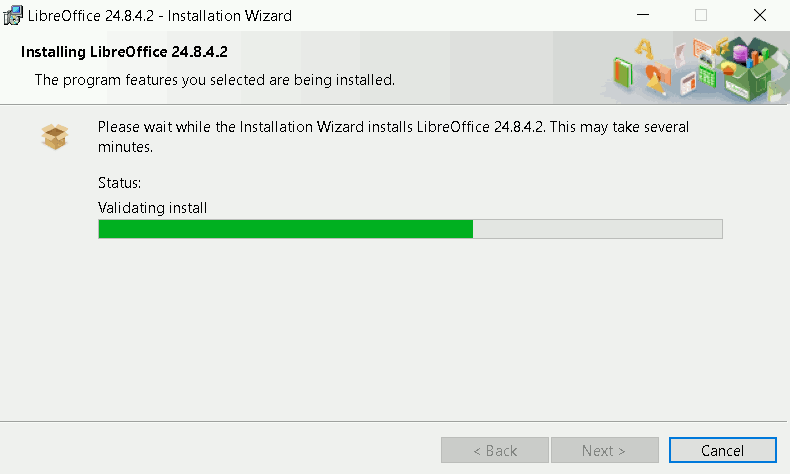
\includegraphics[width=0.7\linewidth]{\currentDir/installingLibreOfficeWindows15installing}}}%
%
\floatRowSep%
%
\subfloat[][%
Under some circumstances, e.g., if you have the Acrobat Reader installed, it may be necessary that the installer does some complex updating. %
It is best to keep the option \emph{Do not close applications. A reboot will be required to complete the setup.} %
So we just click~\menu{OK}. %
On your system, maybe this screen does not appear.%
\label{fig:installingLibreOfficeWindows16needsReboot}%
]{\tightbox{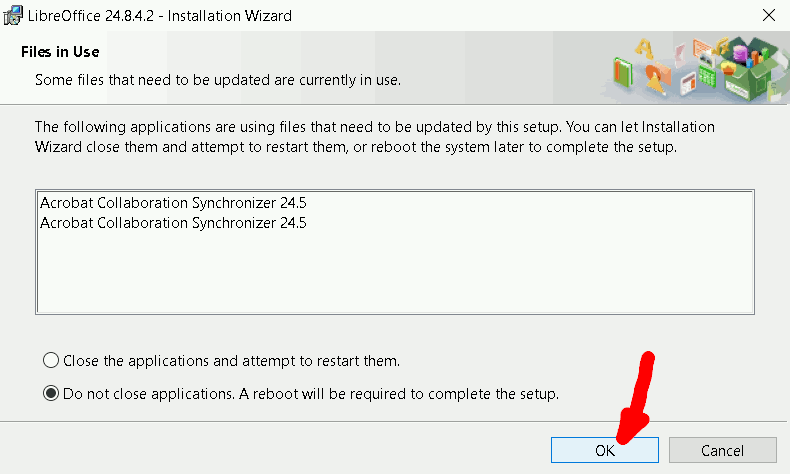
\includegraphics[width=0.7\linewidth]{\currentDir/installingLibreOfficeWindows16needsReboot}}}%
%
\caption{Installing \libreoffice\ under \microsoftWindows~(Continued).}%
\label{fig:installingLibreOfficeWindowsE}%
\end{figure}%
%
%
\begin{figure}%
\ContinuedFloat%
\centering%
%
\subfloat[][%
The installation continues.%
\label{fig:installingLibreOfficeWindows17installing}%
]{\tightbox{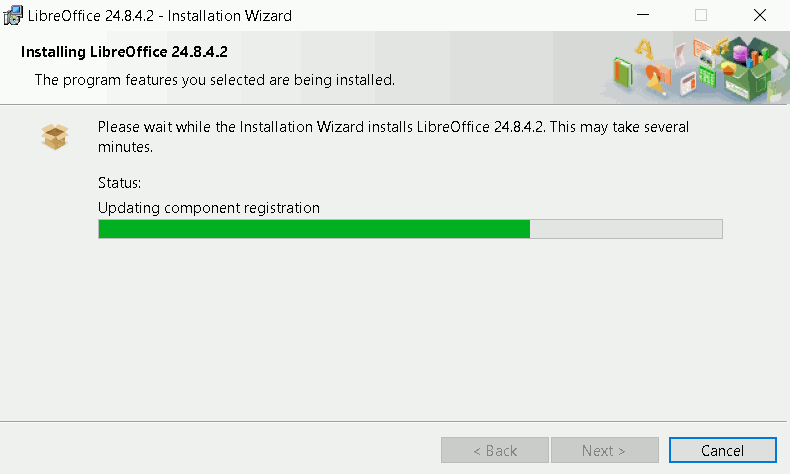
\includegraphics[width=0.7\linewidth]{\currentDir/installingLibreOfficeWindows17installing}}}%
%
\floatRowSep%
%
\subfloat[][%
The installation is completed. %
We click~\menu{Finish}.%
\label{fig:installingLibreOfficeWindows18finish}%
]{\tightbox{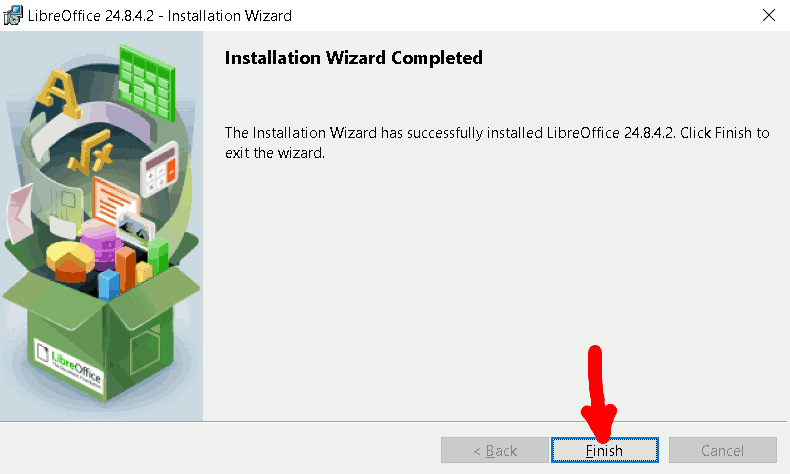
\includegraphics[width=0.7\linewidth]{\currentDir/installingLibreOfficeWindows18finish}}}%
%
\floatRowSep%
%
\subfloat[][%
It may be necessary to reboot~(see \cref{fig:installingLibreOfficeWindows16needsReboot}). %
If so, close all other programs and click~\menu{Yes}.%
\label{fig:installingLibreOfficeWindows19restartNow}%
]{\tightbox{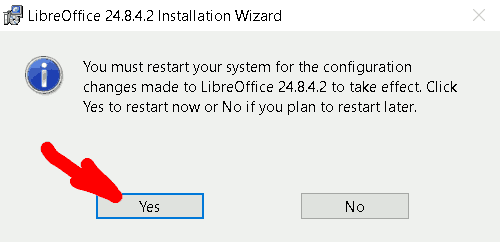
\includegraphics[width=0.56\linewidth]{\currentDir/installingLibreOfficeWindows19restartNow}}}%
%
\floatSep%
%
\subfloat[][%
The restart screen appears%
\label{fig:installingLibreOfficeWindows20restarting}%
]{\tightbox{
\includegraphics[width=0.42\linewidth]{\currentDir/installingLibreOfficeWindows20restarting}}}%
%
\caption{Installing \libreoffice\ under \microsoftWindows~(Continued).}%
\label{fig:installingLibreOfficeWindowsF}%
\end{figure}%
%
%
\begin{figure}%
\ContinuedFloat%
\centering%
%
\subfloat[][%
We can now find a \libreoffice\ icon on the desktop and click on it.%
\label{fig:installingLibreOfficeWindows21afterRestart}%
]{\tightbox{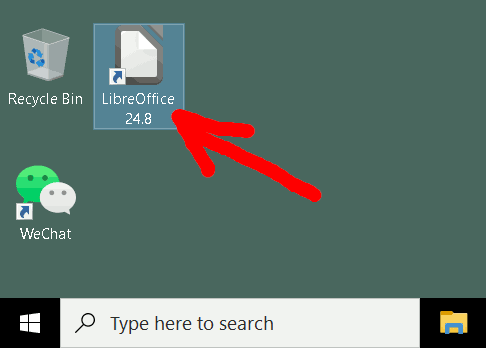
\includegraphics[width=0.6\linewidth]{\currentDir/installingLibreOfficeWindows21afterRestart}}}%
%
\floatRowSep%
%
\subfloat[][%
The \libreoffice\ splash screen appears.%
\label{fig:installingLibreOfficeWindows22startingLibreOffice}%
]{\tightbox{
\includegraphics[width=0.7\linewidth]{\currentDir/installingLibreOfficeWindows22startingLibreOffice}}}%
%
\floatRowSep%
%
\subfloat[][%
We may get asked to set \libreoffice\ as default program to open some file types. %
In order to not mess with your existing system configuration, we un-check the \emph{Perform check on startup} box and click~\menu{Cancel}.
\label{fig:installingLibreOfficeWindows23noCheckOnStartup}%
]{\tightbox{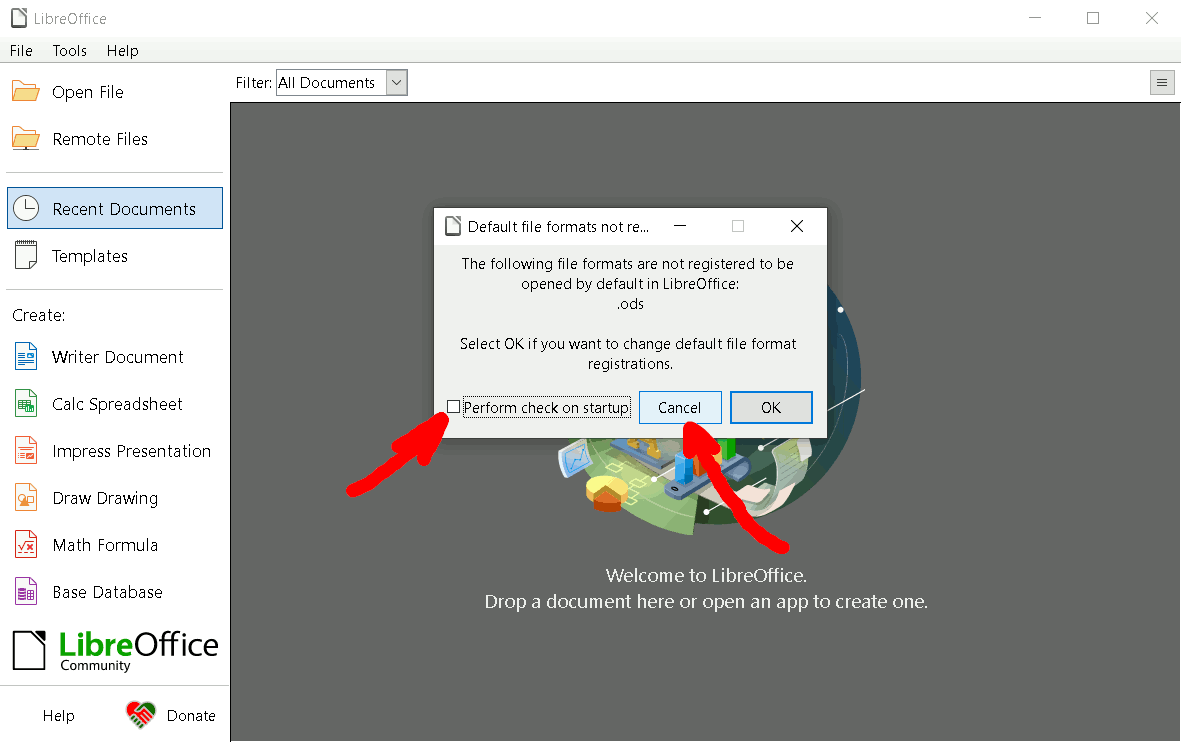
\includegraphics[width=0.7\linewidth]{\currentDir/installingLibreOfficeWindows23noCheckOnStartup}}}%
%
\caption{Installing \libreoffice\ under \microsoftWindows~(Continued).}%
\label{fig:installingLibreOfficeWindowsG}%
\end{figure}%
%
%
\begin{figure}%
\ContinuedFloat%
\centering%
%
\subfloat[][%
We click on the \menu{Base Database} icon in the menu bar on the left-hand side and arrive in the \libreofficeBase\ welcome screen. %
We are done here for now and close the program.%
\label{fig:installingLibreOfficeWindows24db}%
]{\tightbox{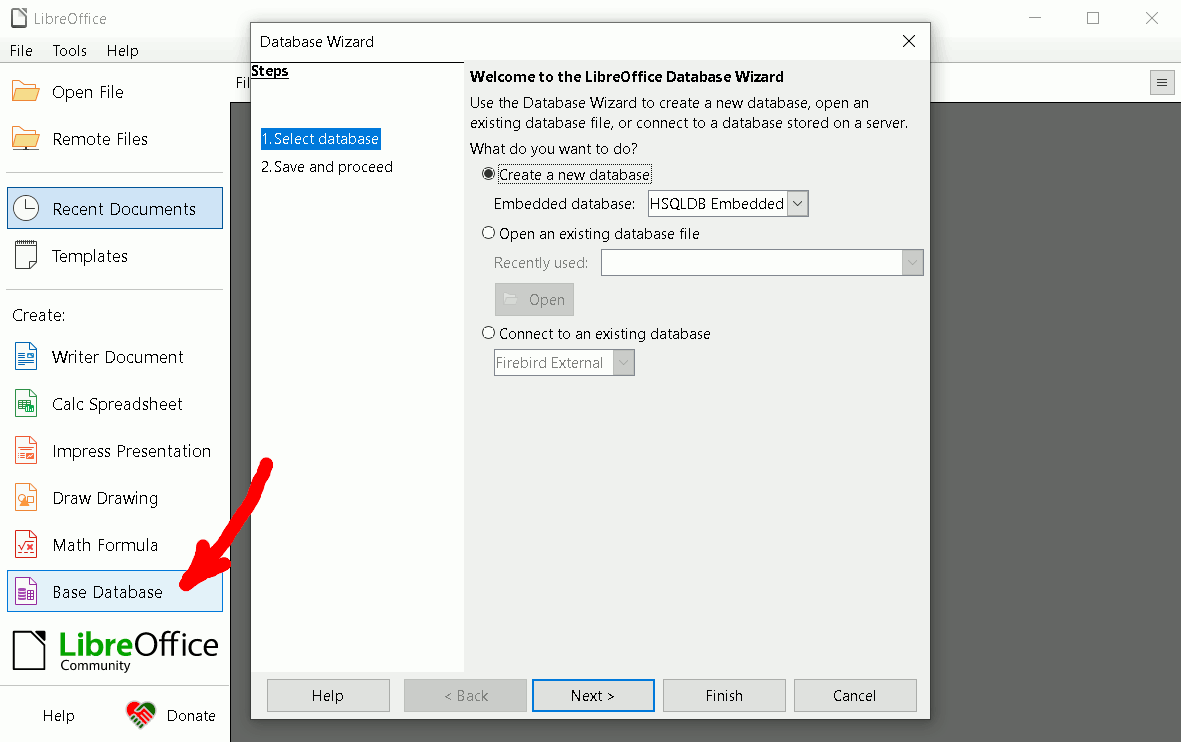
\includegraphics[width=0.7\linewidth]{\currentDir/installingLibreOfficeWindows24db}}}%
%
\caption{Installing \libreoffice\ under \microsoftWindows~(Continued).}%
\label{fig:installingLibreOfficeWindowsH}%
\end{figure}%
%
%
Installing \libreoffice\ under \microsoftWindows\ requires us to first download the software and then to install it.
We therefore open a web browser and go to \url{https://libreoffice.org} in \cref{fig:installingLibreOfficeWindows01website}.
There, we click on \menu{DOWNLOAD}.
A drop-down menu opens in \cref{fig:installingLibreOfficeWindows02download}.
We click on~\menu{Download LibreOffice}.
This takes us to the download page, where we, again, click on~\menu{DOWNLOAD} in \cref{fig:installingLibreOfficeWindows03downloadPage1}.
On this page, we could probably select the operating system of our choice.
Unless you are using some other operating system, the default choice, \menu{Windows (64-bit)}, is probably correct and we can leave it as is.
This takes us to yet another download page in \cref{fig:installingLibreOfficeWindows04downloadPage2}, where we click the big button for downloading \libreoffice.
Finally, the download starts in \cref{fig:installingLibreOfficeWindows05downloading}.

After the download completes, we click \menu{Open file} in \cref{fig:installingLibreOfficeWindows06open}.
A \microsoftWindows\ loading screen appears in \cref{fig:installingLibreOfficeWindows07starting}.
You see, we downloaded a new program from the internet and not the Microsoft Store.
So this worries our \microsoftWindows\ installation, and it asks whether we \emph{really} want to install this program in \cref{fig:installingLibreOfficeWindows08msStore1}.
In \cref{fig:installingLibreOfficeWindows09msStore2}, we click on ~\menu{Install anyway}.

The installation wizard window appears and we click~\menu{Next} in \cref{fig:installingLibreOfficeWindows10wizard}.
On the next screen, we can choose whether we want to customize the installation of \libreoffice\ or, instead, would prefer a \inQuotes{typical}.
We indeed prefer the \inQuotes{typical installation} and click~\menu{Next} in \cref{fig:installingLibreOfficeWindows11wizardTypical}.
In the next screen in \cref{fig:installingLibreOfficeWindows12wizardStartInstall} we confirm that we are also OK with a shortcut on our desktop and click~\menu{Install}.

Now The installation begins~(see \cref{fig:installingLibreOfficeWindows13installStart}).
Since the installer tries to modify our system, \microsoftWindows\ asks us whether we would like to permit the installer to make changes to our system.
We indeed are OK with that, so we click~\menu{Yes} in \cref{fig:installingLibreOfficeWindows14permitChanges}.
The installation continues in \cref{fig:installingLibreOfficeWindows15installing}.

Under some circumstances, e.g., if you have the Acrobat Reader installed, it may be necessary that the installer does some complex updating.
It is best to keep the option \emph{Do not close applications. A reboot will be required to complete the setup.}
I also tried the other option, but that leads to errors down the line.
It is best to leave this at the default setting.
So we just click~\menu{OK} in \cref{fig:installingLibreOfficeWindows16needsReboot}.
On your system, maybe this screen does not appear.
Maybe you do not have Adobe Acrobat installed, maybe you have a different version or setup.
Thus, maybe you will never see this screen and, as a result, do not need to reboot later.
If so, good for you.
If you see the screen, then just accept that you will need to reboot eventually.

Either way, the installation continues in \cref{fig:installingLibreOfficeWindows17installing}.
And eventually, it is completed and we click~\menu{Finish} in \cref{fig:installingLibreOfficeWindows18finish}.
At this stage, if you did see the screen from \cref{fig:installingLibreOfficeWindows16needsReboot}, it becomes necessary to reboot.
If so, you should close all other programs and click~\menu{Yes}, as shown in \cref{fig:installingLibreOfficeWindows19restartNow}
Then, the restart screen appears in \cref{fig:installingLibreOfficeWindows20restarting}.

Regardless whether you needed to reboot or not, we can now find a \libreoffice\ icon on the desktop, as shown in~\cref{fig:installingLibreOfficeWindows21afterRestart}.
We click on it.
The \libreoffice\ splash screen appears in \cref{fig:installingLibreOfficeWindows22startingLibreOffice}.
We may get asked to set \libreoffice\ as default program to open some file types.
In order to not mess with your existing system configuration, we un-check the \emph{Perform check on startup} box and click on~\menu{Cancel} in \cref{fig:installingLibreOfficeWindows23noCheckOnStartup}.

We now click on the \menu{Base Database} icon in the menu bar on the left-hand side and arrive in the \libreofficeBase\ welcome screen in \cref{fig:installingLibreOfficeWindows24db}.
We are done here for now and close the program.
We have downloaded and installed \libreofficeBase\ and can use it for our experiments later.%
%
\FloatBarrier%
\endhsection%
%
